% Chapter 1

\chapter{Introduction and Dataset} % Main chapter title

\label{Chapter1} % For referencing the chapter elsewhere, use \ref{Chapter1} 

%----------------------------------------------------------------------------------------

% Define some commands to keep the formatting separated from the content 
\newcommand{\keyword}[1]{\textbf{#1}}
\newcommand{\tabhead}[1]{\textbf{#1}}
\newcommand{\code}[1]{\texttt{#1}}
\newcommand{\file}[1]{\texttt{\bfseries#1}}
\newcommand{\option}[1]{\texttt{\itshape#1}}

%----------------------------------------------------------------------------------------

\section{Introduction}

Since the appearance of the powerful baseline system known as Fully Convolutional Network (FCN) \parencite{Reference1} several structures have been developed using the power of convolutions and avoiding the use of fully connected structures. For example, structures such as \parencite{Reference2} or \parencite{Reference3}, which are built for both tasks of detection and segmentation using CNN as main feature extractor. As another important example, structures initially designed for detection, such as Mask R-CNN \parencite{Reference4}, use FCN modules to expand its capacity to do semantic segmentation, or in this case, instance segmentation. Also, among the structures that use CNN as its main core,  stand out structures specific for semantic segmentation. These networks can be separated regarding they structural differences and, hence, different groups can be established: encoders-decoders which use pooling layers with skip connections \parencite{Reference5}, \parencite{Reference6} and those which use atrous or dilated convolutions \parencite{Reference7}, among others. As a matter of fact, some of these structures add Conditional Random Fields (CRF) at the end of the network to refine the segmentation prediction, as in \parencite{Reference8}. As seen the variety of application as feature extraction mechanism is outstanding.  \newline

Nevertheless, it is also by the huge variety of applications of these networks and its outstanding performance that they have acquired great popularity. From the well known and established tasks of classification and object detection \parencite{Reference9}, \parencite{Reference10}, to the more recent tasks such as pose estimation \parencite{Reference11} or action recognition \parencite{Reference12}, and even text classification \parencite{Reference13}. Tasks which can be devoted to a wide range of types of data: biological \parencite{Reference14}, aerial \parencite{Reference15} and human \parencite{Reference16} among others.\\

Our purpose is then to study the performance and behavior of fully convolutional networks regarding semantic segmentation but with a specific kind of data: human body parts. For this reason we have chosen the SURREAL data set, \parencite{Reference17}. It provides around 6M frames from synthetically rendered 3D sequences of human motion data. As strong point stands out the variety and quantity of data, in terms of images but also of complementary information such as depth or body part joints. As main drawbacks, the fact that there are not occlusions with the background (human and background are separate layers) and that the footages are single person takes.\\

Considering our purpose, and having into account the limited time and space, several structures are going to be considered. To be able to have a differentiated analysis two different structures, regarding its segmentation procedure, has been selected: SegNet and Image Cascade Network (ICNet), \parencite{Reference18}. Segnet is a encoder-decoder with skip connections that reuse the pooling indexes of the encoder in the decoder part and ICNet is a cascade structure of different resolution branches which merge up to give a final segmentation. As commented, although both structures use CNN as its main component, both differ in the procedure or structure and then a differential study is presumed to be possible to be carried out. Nevertheless, only reference to general segmentation purposed networks has been defined. Among the networks which use CNN as its main component also stand out networks which are specific for certain types of objects. In our case, as we are studying the human body, we are interested in structures that can be specialized to obtain better results when dealing with images that contain such objects. Among these structures  stand out those which use key points or pose information of the body to finally segment it, \parencite{Reference19} and \parencite{Reference20}, and also those which make use of the so called hourglass networks. In our case we have selected the Stacked Hourglass network, \parencite{Reference21}. This decision is based on the supposed ease that the structure will allow for its study and modification to observe the effects on the segmentation of the human body.\newline

As stated, the work will have two main parts: one devoted to general segmentation purposed structures and the other to human body specific structures. However, the procedure to implement them will be the same, that is: after having selected a recent article, an adequate code is searched in Tensorflow. Once the code has been found suitable for the study several changes are applied to it to obtain the desired results.\newline

Concluding the introduction, the purpose and definition of this work is to study the differences in performance  and its reasons of different deep neural networks which are mainly based on CNNs with respect to a specific human body dataset: SURREAL. \\


\section{SURREAL Dataset}

Deep neural structures stand out regarding accuracy results when large amounts of data are available for training. As manual annotation or supervision for obtaining ground truth data for tasks, such as ours, semantic segmentation, is expensive and time consuming, synthetic generation of this data has been used during the past years.\newline

As real images are rich detailed in terms of textures, light, occlusions, shapes, the main problem regarding synthetic generation of data has been the reality of the images rendered. For this purpose, and as our task is semantic segmentation, we have chosen the SURREAL dataset (Synthetic hUmans foR REal tasks). The main reason is that it has a rich per-pixel ground-truth  allowing the adequate training for tasks such as ours. As is stated in the original paper, the rendering is sufficiently realistic to allow knowledge transfer from the synthetic training images to testing real RGB images. \newline

The resulting dataset consists of 6.5 million frames grouped into 67582 continuous image sequences of size 320x240. As the data is synthetically generated, ground truths regarding optical flow, body part segmentation, depth, 3D and 2D joints and surface normals are also generated.
 
\subsection{Image rendering procedure}

The three main components of the data generation are: the creation of the synthetic body using the SMPL (a skinned multi-person linear model) body model, the fitting of its parameters by MoSH (Motion and shape capture from sparse markers), and the final rendering of the image from 3D sequences of motion capture (MoCap) data. The final results is a 3D human body with a random pose, random shape, random texture and rendered form a random point of view, random lightning and random background.\newline

The main steps or components in the rendering or generating procedure are: body model, body shape, body pose, texture, light, camera, background and ground truth. The body model is initially defined using SMPL which decomposes body deformations into shape and pose. Shape is adjusted using a random sample from the CAESAR dataset and approximating it using SMPL shape components. Following, pose is fitted using as a reference a MoCap sequence and the 3D location of body markers that it has. The fitting is carried out by MoSh since transferring MoCap 3D data to a new model appears to be challenging. Next, two types of textures are used in the rendering process: the first one, which uses CAESAR scans and lacks of resolution and texture variety, and the second, extracted from 3D scans of subjects with normal clothing. All this rendering process for each image sequence is carried out with fixed light and camera conditions.\newline 

Regarding light the body is illuminated using Spherical Harmonics which coefficients are randomly sampled from a uniform distribution. In the case of the camera it is located for the viewpoint  to point at the pelvis of the figure, positioned at a random distance and  with random yaw angle. For the background, the person is rendered in top of a static image extracted from the LSUN dataset also to avoid having other human figures in the background. Finally, through different renderings of the image and the whole sequence through Blender all the ground truths are extracted and determined.

\subsection{Dataset details and adaptation}

The dataset is organized as the traditional package of training, validation and test data. The important unit of information is composed by 4 files: an \textit{.mp4} image sequece (video), a segmentation, a depth and info files (in \textit{Matlab} form, \textit{.mat}). All these matrices include both ground truths and characteristics of the video sequence. Sequences are grouped regarding the characteristics of the pose and optical flow.\newline

In each of the these categories (training, validation and test) there are 3 different partitions that reproduce the same sequences but with a main different characteristic: the overlap between one video sequence and the next is different. That is, in the first one we have a 30$\%$ overlap between consecutive sequences in the same group, and in the second a 50$\%$, and a 70$\%$ in the third. Also, between them are differences regarding background, light, camera orientation and texture but not pose. \newline

To obtain the final images and their ground truths we have followed a specific procedure and several modifications. First of all, in each segmentation \textit{mat} file are found as much matrices as frames have the corresponding video sequence. What has been done is to cut the video in frames and then all this frames have been saved as \textit{jpg} images. Then each of the ground truth matrices in the segmentation file has been rendered as an image in the \textit{png} format (this is very important since the \textit{jpg} format for compressing an image changes the values of it and hence if the ground truth is saved in \textit{jpg} the ground truth values are changed and its functionality broken). Then what is had is an RGB image and its associated segmentation ground truth with an integer value at each pixel ranging from 0 to 24 (the delimited body parts). \newline

Secondly, after having all the images and ground truths in the adequate format we have selected a cluster of approx. 90k images for training from the 50$\%$ overlapping group, 15k for validation and 15k for testing. The clustering operation has been executed taking into account the 3D joints data of each of the bodies in the images.\newline

Thirdly, to center the attention in the human body and taking into account that the background is static and plays no role further than background (no occlusions, nor human in the background) the images have been cropped. The procedure has been the following: the box that the body occupies is determined, the longer dimension of the box is selected, then an extra value is added to this dimension. This final length value is used for replacing the other shorter side of the box leaving a squared box which contains the human body inscribed in a reduced background with respect to the original image. Other informative quantities such as coordinates of joints in the image has been moved accordingly to this transformation. \newline

Finally, another operation on the image is needed to have the images ready used for training, validating and testing. The fact is that in the original ground truths there were some errors in the labels assigned to the chest and pelvis zones. In these zones there were pixels that had the head label assigned. Hence, the points had to be refilled with the appropriate values corresponding to each zone. The process used to achieve this was: select connected components with the label head, select all the areas except the bigger one (the head), and then using 8-connectivity to refill the erroneous points with the maximum occurring value in their neighborhood.\newline

After all this procedure, the cluster images were prepared for training, validating and testing. In Fig \ref{dataset:samples} examples of the images and their respective ground truths can be observed.

\begin{figure}
\centering
\begin{subfigure}{.19\textwidth}
\centering
  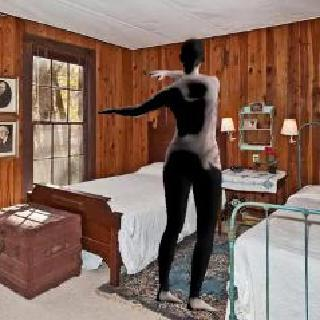
\includegraphics[scale=0.3]{80_15_c0002_85.jpg}
\end{subfigure}
\begin{subfigure}{.19\textwidth}
  \centering
  
\includegraphics[scale=0.3]{ung_77_09_c0001_67.jpg}
\end{subfigure}
\begin{subfigure}{.19\textwidth}
  \centering
  
\includegraphics[scale=0.3]{ung_91_62_c0003_87.jpg}
\end{subfigure}
\begin{subfigure}{.19\textwidth}
  \centering
  
\includegraphics[scale=0.3]{ung_144_02_c0006_2.jpg}
\end{subfigure}\\
\begin{subfigure}{.2\textwidth}
\centering
  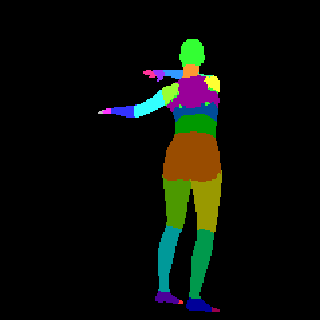
\includegraphics[scale=0.3]{80_15_c0002_segm_85.png}
\end{subfigure}%
\begin{subfigure}{.19\textwidth}
  \centering
  
\includegraphics[scale=0.3]{ung_77_09_c0001_segm_67.png}
\end{subfigure}
\begin{subfigure}{.19\textwidth}
  \centering
  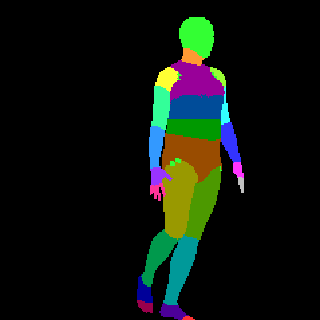
\includegraphics[scale=0.3]{ung_91_62_c0003_segm_87.png}
\end{subfigure}
\begin{subfigure}{.19\textwidth}
  \centering
  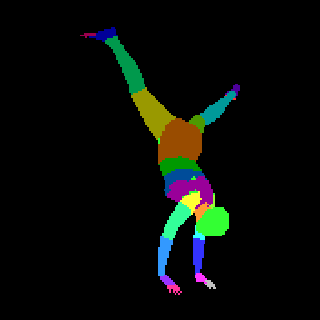
\includegraphics[scale=0.3]{ung_144_02_c0006_segm_2.png}
\end{subfigure}

\caption{First row: sample images. Second row: corresponding ground truths}
\label{dataset:samples}
\end{figure}
